%%%%%%%%%%%%%%%%%%%%%%%%%%%%%%%%%%%%%%%%%
% Short Three-Column Newsletter
% LaTeX Template
% Version 1.0 (11/9/13)
%
% Original author:
% Frits Wenneker (http://www.howtotex.com) 
% With extensive modifications by:
% Vel (vel@latextemplates.com)
% 
% This template has been downloaded from:
% http://www.LaTeXTemplates.com
%
% License:
% CC BY-NC-SA 3.0 (http://creativecommons.org/licenses/by-nc-sa/3.0/)
%
%%%%%%%%%%%%%%%%%%%%%%%%%%%%%%%%%%%%%%%%%

%----------------------------------------------------------------------------------------
%	PACKAGES AND DOCUMENT CONFIGURATIONS
%----------------------------------------------------------------------------------------

\documentclass[10pt,a4paper,ngerman,twoside]{article} % Paper type (a4paper, usletter or legal) and font size (10, 11 or 12)

%\setlength\topmargin{-80mm} % Top margin
\setlength\topmargin{-48pt} % Top margin
\setlength\headheight{0pt} % Header height
\setlength\textwidth{7.0in} % Text width
\setlength\textheight{9.5in} % Text height
\setlength\oddsidemargin{-30pt} % Left margin
\setlength\evensidemargin{-30pt} % Left margin (even pages) - only relevant with 'twoside' article option
%\setlength\inner{4cm}
%\setlenfth\outer{2cm}
%\usepackage{geometry}
%\geometry{bindingoffset=20mm}
%\setlength\bindingoffset{2cm}

\usepackage{charter} % Charter font for main content

\frenchspacing % Reduces space after periods to make text more compact for a three-column layout
\usepackage{babel}
\usepackage[utf8]{inputenc}
\usepackage{graphicx} % Required for including images
\usepackage{amssymb} % Math packages
\usepackage{amsmath} 
\usepackage{multicol} % Required for the three-column layout of the document
\usepackage{url} % Clickable links
\usepackage{enumitem} % Reduces the amount of space within and between lists with [noitemsep,nolistsep]
\usepackage{marvosym} % Required for the use of symbols
\usepackage{wrapfig} % Allows wrapping text around figures
%\usepackage[T1]{fontenc} % Use 8-bit encoding that has 256 glyphs
\usepackage{datetime} % Required for defining a custom date style
\newdateformat{mydate}{\monthname[\THEMONTH] \THEYEAR} % Set a custom date format
\usepackage[pdfpagemode=FullScreen, colorlinks=false]{hyperref} % Link colors and PDF behavior in Acrobat
\usepackage{fancyhdr} % Required to define custom headers/footers
\usepackage{hyperref} % funktioniert nicht ?
\pagestyle{fancy} % Enables the custom headers/footers for all pages following this

%-----------------------------------------------------------
% Header and footer
\lfoot{\footnotesize % Left footer containing newsletter contact information
%\begin{wrapfigure}{l}{2.0cm}
%
\includegraphics[width=2cm]{ccbysa88x31.png} 
%\end{wrapfigure}
R.I.S. Journal Ausgabe 001, Jänner 2014: \textbf{R}emix, \textbf{I}mprove, \textbf{S}hare. Das freie, creativ-commons lizensierte Journal.  \\
\Mundus\ Download und andere Formate: \href{http://spielend-programmieren.at/de:ris:start}{\texttt{spielend-programmieren.at/de:ris:start}} \quad
%\Telefon\ (000) 111-1111 \quad
\Letter\ \href{mailto:horst.jens@spielend-programmieren.at}{horst.jens@spielend-programmieren.at}
}

\cfoot{} % Empty center footer

\rfoot{\footnotesize ~\\ Seite \thepage} % Right footer - page counter

\renewcommand{\headrulewidth}{0.0pt} % No horizontal rule for the header
\renewcommand{\footrulewidth}{0.4pt} % Horizontal rule separating the footer from the document
%-----------------------------------------------------------

%-----------------------------------------------------------
% Define separators
\newcommand{\HorRule}[1]{\noindent\rule{\linewidth}{#1}} % Creates a horizontal rule
\newcommand{\SepRule}{\noindent	% Creates a shorter separator rule
\begin{center}
\rule{250pt}{1pt} % Page width and rule width
\end{center}
}
\newcommand{\Trenner}{\noindent
\begin{center}
\rule{100pt}{1pt}
\end{center}
}
%-----------------------------------------------------------

%-----------------------------------------------------------
% Define title and article styles
\newcommand{\NewsletterName}[1]{ % Newsletter title
\begin{center}
\Huge \usefont{T1}{fvs}{b}{n} % Use the Bera Sans Bold font
#1
\end{center}	
\par \normalsize \normalfont}

\newcommand{\JournalIssue}[1]{ % Date and issue number at the top of the newsletter
%\hfill \textsc{\mydate \today, No #1} % Right-aligned date and issue number
\hfill \textsc{Jänner 2014, Ausgabe 001}
\par \normalsize \normalfont}

\newcommand{\NewsItem}[1]{ % News item title
\usefont{T1}{fvs}{n}{n} % Use the Bera Sans Normal font
\vspace{24pt}\large #1\vspace{3pt} % Print the title with space around it in a larger font size
\par \normalsize \normalfont}

\newcommand{\NewsAuthor}[1]{ % Author name under the item title
\hfill von \textsc{#1} \vspace{20pt} % Right-aligned author name in small caps with space after it
\par \normalfont}		

%----------------------------------------------------------------------------------------
%	TITLE
%----------------------------------------------------------------------------------------

\begin{document}

\JournalIssue{1} % Issue number
\NewsletterName{R.I.S. Journal} % Newsletter title
%\begin{center}
%\textbf{R}emix \textbf{I}mprove \textbf{S}hare - das freie Journal für Open Source Education
%\end{center}
\noindent\HorRule{3pt} \\[-0.75\baselineskip] % Thick horizontal rule
\HorRule{1pt} % Thin horizontal rule



%\setlength{\columnsep}{16pt} % Uncomment to manually change the white space between columns
%\begin{multicols}{3} % Begin the three-column layout

%----------------------------------------------------------------------------------------
%	OTHER NEWS
%----------------------------------------------------------------------------------------
%-----------------------------------------------------------
%
%-----------------------------------------------------------
%RIS-Journal Titel (Titelgrafik hier einfügen)
\begin{multicols}{3}
\NewsItem{}
\section*{Pyladies Vienna}
\label{floor}
\NewsAuthor{Floor DREES und Horst JENS}
\begin{center}

\includegraphics[width=\linewidth]{floor/floor.jpg} \\
\footnotesize{Floor Drees. Bildrechte. Floor [1]}
\end{center}
\textbf{Floor Drees [1], Gründerin der Lerngruppe Pyladies Vienna [2], beantwortete in diesem Email-Interview Fragen zur über die Programmiersprache Python [3] / über Pyladies, zum Unterschied zwischen Holland und Österreich sowie zur Situation von Frauen in der IT-Branche. Übersetzung von Horst JENS [4]} \\
\begin{center}

\includegraphics[width=\linewidth]{floor/floorlogo.png} \\
\footnotesize{Logos von python und pyladies. Bildrechte: [3], [2]}
\end{center}

(Beginn der Übersetzung) \\
\textbf{Horst:} Hallo Floor, bitte erzähl kurz über dich. Wo bist du her, warum bist du in Wien, wovon lebst du? \\
\textbf{Floor:} Hallo. Naja, ich studierte Grafik Design in Rotterdam und arbeitete dort einige Jahre als \textbf{Community Managerin} bevor ich nach Wien zog um in einem \textbf{Startup} zu arbeiten.  Ich sagte mir ich bleibe für vielleicht ein Jahr in Wien, aber es wurden zweieinhalb Jahre daraus. Vor zwei Wochen übersiedelte ich nach Berlin. Seit ich nach Wien zog hat sich viel verändert. 

Ich begann mich fürs Programmieren zu interessieren, ich begann CSS, Ruby und Python zu lernen und ich bekam einen Job als \textbf{'Developer evangelist'} bei \href{http://www.checkio.org/}{\textit{CheckiO [5]}}, einer Spiele-Plattform für Programmierer. Ich liebe es Kommunikationsfähigkeiten mit technischen Skills zu kombinieren, und Dank der Arbeit bei CheckiO (\textbf{gamified learning}) konnte ich meine Coding-Skills ordentlich verbessern! \\
\textbf{Horst:} Was ist für dich der auffälligste Unterschied bei Land und Leuten zwischen Holland (bzw. anderen Ländern) und Österreich, deiner Erfahrung nach ? \\
\textbf{Floor:} Was ich als größten Unterschied erlebt habe generell ist die 'Schau ma mal..' Mentalität hier. Ich kann ziemlich enthusiastisch (excited) werden für ein Projekt und mag sofort loslegen. Die meisten Österreicher sind mehr... konservativ, schätze ich. Vielleicht sind Holländer einfach nur direkter. Ich hatte das Gefühl sobald ich jemanden gefunden hatte der gern mit mir arbeitet waren sie (die Österreicher) voll dabei. Es hat nur ein bisserl länger gebraucht. \\
\textbf{Horst:} Warum sollten junge Leute (speziell Mädchen) programmieren lernen ? \\
\textbf{Floor:} Ich denke die Fähigkeit zu programmieren ist DER 'Skill' der Zukunft. So wie die Baby-Boomer lernen mussten mit all den Computer um sie herum umzugehen. 

Wer das nicht macht würde sich selbst vom Arbeitsmarkt ausschließen. Um von meiner eigenen Erfahrung zu sprechen, ich wurde wesentlich besser in meinem Job als Community-Manager sobald ich lernte die Wünsche der Community den Entwicklern (devs) zu übersetzten. Ich denke es ist eine  wichtige Fähigkeit wenigstens die Grundlagen von Markup und Styling (\textbf{html}, \textbf{css}) zu verstehen, zu wissen was \textit{Backend} passiert und vielleicht leicht verständlichen Programmcode wie \textbf{Ruby} oder \textbf{Python} 'lesen' zu können. 
\begin{center}
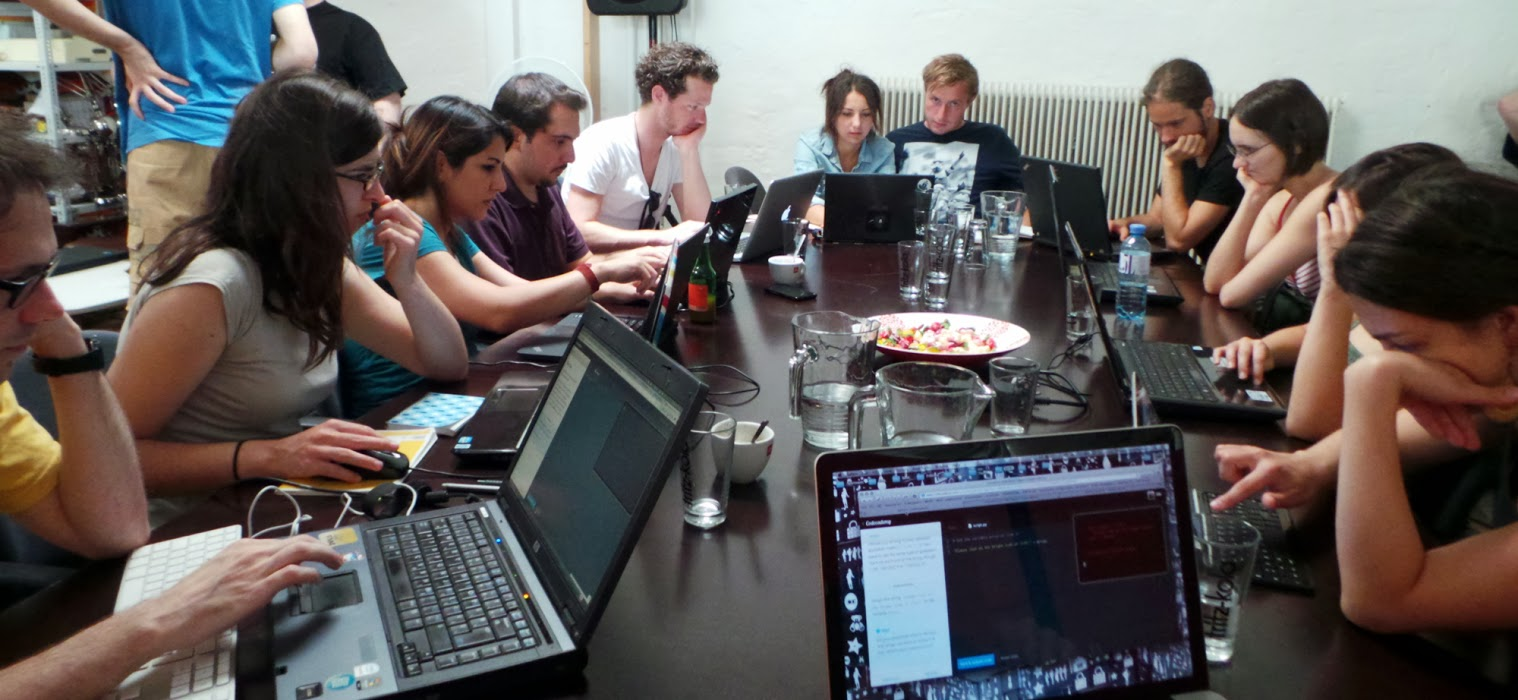
\includegraphics[width=\linewidth]{floor/floor5a.jpg} \\
\footnotesize{Pyladies-Treffen. Bildrechte: [1]} 
\end{center}
Und falls diese Jugendlichen zufällig Mädchen sind und sich für solche Sachen interessieren dann hoffe ich sehr dass sie ihre Studien in diesem Gebiet weiterverfolgen, denn wir brauchen dringend mehr Diversity um bessere Software zu erschaffen! \\
\textbf{Horst:} Was war deine Motivation Programmieren zu lernen ? Hattest du ein (weibliches) Rollenmodell ?
\textbf{Floor:} Das klingt vielleicht lustig, aber ich wollte eigentlich \textbf{Bugs fixen}. Und ich wollte lernen wie man mit den Entwicklern bei dem Startup halbwegs professionell kommuniziert. 
Ich fing an die Rails Girls Tutorials durch zu arbeiten mit einem Arbeitskollegen. Er ist extrem gut mit CSS vertraut und ein sehr geduldiger Typ. Später verbrachte ein anderer Freund und Ex-Arbeitskollegen seine Wochenenden damit mir und einem Freund Ruby beizubringen, \textit{'the test driven way'}. Diese Unterstützung bedeutete enorm viel für mich.
Was ich als Community-Managerin über die Jahre gelernt habe ist dass ein großer Teil der Arbeit darin besteht gut reden zu können ('Talking the Talk'... sich selbst und die eigenen Fähigkeiten verbal präsentieren zu können). Ich begann all die Konferenz-Talks über Programmierung anzuschauen, und ich lauschte dem \href{http://rubyrogues.com/}{\textit{Ruby Rogues Podcast [6]}} inbrünstig. Am Anfang musste ich alle 10 Minuten auf die Pause Taste drücken um die Fachbegriffe nachzuschlagen. Aber nach einer Weile begann ich Dinge im Kopf miteinander zu verbinden und erkannte Begriffe und ich konnte eine ganze Episode ohne Pause anhören. 
All die Jungs und Mädels bei Ruby Rogues wurden für mich zu Vorbildern. Ich mochte speziell Bücher von  Avdi Grimm, (z.B. \href{http://objectsonrails.com/}{\textit{Objects on Rails [7]}} oder \href{http://www.confidentruby.com/}{\textit{Confident Ruby [8]}}) 
. Seine Bücher habe ich von vorne bis hinten gelesen. Und auch \href{http://kytrinyx.com/}{\textit{Katrina Owen [9]}}). \\
\begin{center}

\includegraphics[width=\linewidth]{floor/floor-ruby.png} \\
\footnotesize{Confident Ruby. Bildrechte: [8]} \\
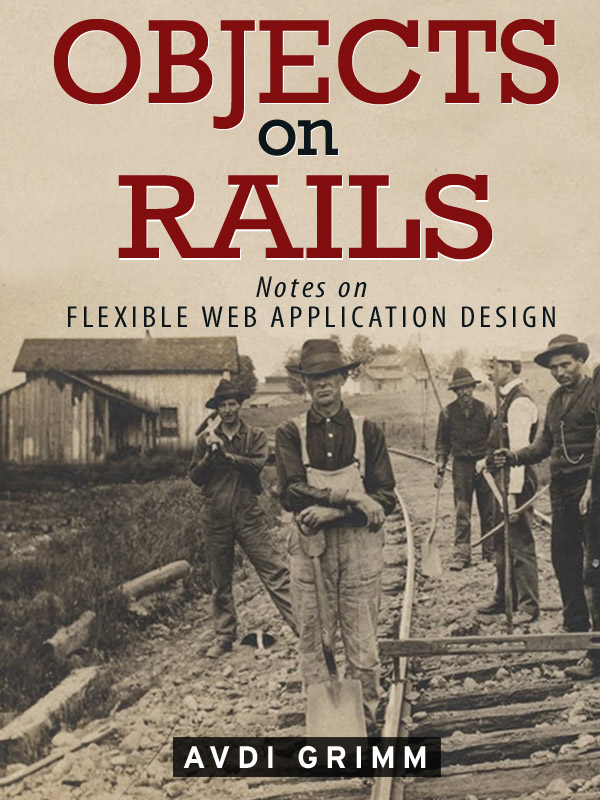
\includegraphics[width=\linewidth]{floor/floor-rails.jpg} \\
\footnotesize{Objects on Rails. Bildrechte: [7]} 
\end{center}
\textbf{Horst:} Deine erste Programmiersprache war ? \\
\textbf{Floor:} Zuerst probierte ich mit PHP herum als ich anfing mit WordPress zu arbeiten. Ich war damals 18 Jahre alt oder so. Aber das war mehr ein löschen, reloaden und schauen-was-passiert Ansatz ! \\
\textbf{Horst:} Warum Python ? \\
\textbf{Floor:} Ich arbeite für mehrere Startups die Python verwendeten, und ich hatte mit Django zu tun, sodass es logisch war dass Python als nächstes auf meine Liste kam. Und, nicht zu vergessen, Python Erfinder Guido van Rossum ist Holländer ! \\
\textbf{Horst:} Was ist Pyladies Vienna? \\
\textbf{Floor:} Immer wenn ich etwas neues lerne brauch ich ...sozialen Druck. Alleine lernen kann sehr öde sein und ich wollte andere AnfängerInnen finden die den Samstag mit mir gemeinsam verbringen wollten um zu lernen. Deshalb organisierte ich einen ersten Workshop, suchte mir ein Tutorial aus, besorgte Kekse und legte los.

Dass ich eine Pyladies Gruppe (chapter) gründete war eher Zufall. Ich las über diese internationale Bewegung und dachte mir dass diese Marke zu übernehmen ('franchising this brand') würde mir dabei helfen TeilnehmerInnen und Unterstützung zu finden. Was funktionierte.
Ich bin sehr zuversichtlich dass PyLadies Vienna weiterhin wachsen wird, mit Laura als neuer Anführerin und dass die geplante Zusammenarbeit mit Laber's Lab (die haben die Arduino bootcamps in Wien organisiert) funktionieren wird. \\
\textbf{Horst:} Deine Meinung zu anderen Programmiersprachen ? \\
\textbf{Floor:} Ich beschäftige mich in letzter Zeit mit JavaScript, und ich verfluche mich dass ich nicht schon viel früher damit begonnen habe. Es macht Spaß - manchmal. Für ein Nebenprojekt musste ich etwas Java lernen und mochte das auch. Sicher, Java ist umständlich und man muss sehr viele Programmzeilen schreiben damit man ein Resultat sieht... aber Java hat seine Verdienste. Ich mag dieses 'language bashing' gar nicht dass man manchmal auf Konferenzen sieht. Es ist so unnötig. \\
\textbf{Horst:} Deine Erfahrung mit Frauen in der Technik ? \\
\textbf{Floor:} Generell gibt's da zu wenig Frauen - haha ! Aber immer wenn ich Entwicklerinnen (female developers) kennen lerne ('they are usually super excited about coding') sind die begeistert vom Programmieren und dieser Enthusiasmus ist ansteckend. \\
\textbf{Horst:} Warum glaubst du gibt es hauptsächlich männliche Programmierer in Österreich (anderen Ländern) ? \\
\textbf{Floor:} Ich persönlich denke -und vielleicht liege ich falsch- dass Informatik als Fach in den Schulen nicht sehr attraktiv für Mädchen ist. Ich war wirklich schlecht in Mathematik und habe die Aufgaben nie interessant gefunden. Warum soll ich die Wahrscheinlichkeit, eine rote Murmel aus einem Sack zu ziehen, ausrechnen ? Ich durstete nach Beispielen aus dem echten Leben. Unsere Informatikstunden ertranken in Mathematik-Rätseln, ich hätte wirklich gerne gelernt wie man Homepages selber macht (HTML, CSS, vielleicht JavaScript). Etwas machen wo man -nach Knopfdruck- die Früchte der eigenen Arbeit bewundern kann, dass hätte mich total fasziniert. 

Mir fällt auf dass auf den Rails Girls Workshops wo ich unterrichte (und die ich organisiere) die meisten Teilnehmerinnen ebenfalls dieses sofortige Feedback suchen. \\
\textbf{Horst:} Dein schlimmstes Vorurteils-Erlebnis (in Bezug auf Frauen in Technik) ? Welche typische Aussage nervt dich speziell ? \\
\textbf{Floor:} 'Wenn sie (Frauen) sich (für Technik) interessieren würden dass wärens sie hier. Wir sind offen für alle'. Das ist soooo vergiftet. Viele Frauen die mit Programmieren anfangen sind schon etwas älter weil sie in der Schule nie dafür interessiert wurden. Manchmal sind sie oder fühlen sie sich wie Anfängerinnen. Wenn sie dann bilder sehen von Meetings mit gegen 100\% Männeranteil dann wirkt das nicht sehr einladend. Du fürchtest dich dass deine Fähigkeiten in Frage gestellt werden. Was manchmal auch passiert. Bestes Beispiel: Oft kommen neue Leute zum Vienna.rb (Ruby) Meeting die ich mitorganisiere. Bis die Leute sehen dass ich den Eröffnungsvortrag halte glauben sie ich bin die Servierkraft vom Catering. Das ist nicht cool, aber ich kann meistens drüber lachen. \\
\textbf{Horst:}  Dein bestes Technik/Gender Erlebnis ? \\
\textbf{Floor:} Ich finde die Ruby/Rails Gemeinschaft als Ganzes sehr einladend. Ich teile mit anderen meine Code Schnipsel, oder erzähle welches Buch ich gerade lese, und ich bekomme super nettes Feedback via Twitter. Vielleicht spielen Rails Girls und Railsbridge eine große Rolle dabei ein so sicheres Umfeld zu schaffen.

Als ich neulich fragte wer mit mir zusammen an einem Javascript Projekt zu arbeiten will bekam ich auch extra nette Antworten. \\
\textbf{Horst:} Welchen Rat hast du für junge (Schul)Mädchen die sich für eine Programmier-Karriere interessieren ? \\
\textbf{Floor:} Du fragst eine Kunststudentin die Social-Media-Managerin wurde um dann eine Kehrtwendung zu machen und Webseiten zu erstellen! Mein Rat: 

Folge deinem Herz, da draußen gibt es Resourcen die dir helfen werden wenn du deine Meinung änderst und etwas anderes lernen willst. Und ich hoffe du bewahrst dir Offenheit und eine gesunde Person Neugier (aufs Programmieren natürlich!). \\
\textbf{Horst:} Letzte Lebensweisheiten für unsere jungen LeserInnen ? \\
\textbf{Floor:} Was sie dir in der Schule beibringen ist wie man sich Wissen aneignet, nicht endgültiges Wissen. Da draußen gibt es so viel, benutze deine Fähigkeiten um etwas zu lernen was DU nützlich und interessant findest. Oft wirst du Leute finden die dich dabei anleiten, vielleicht sogar deine Lehrer!

(Ende der Übersetzung)
\begin{center}
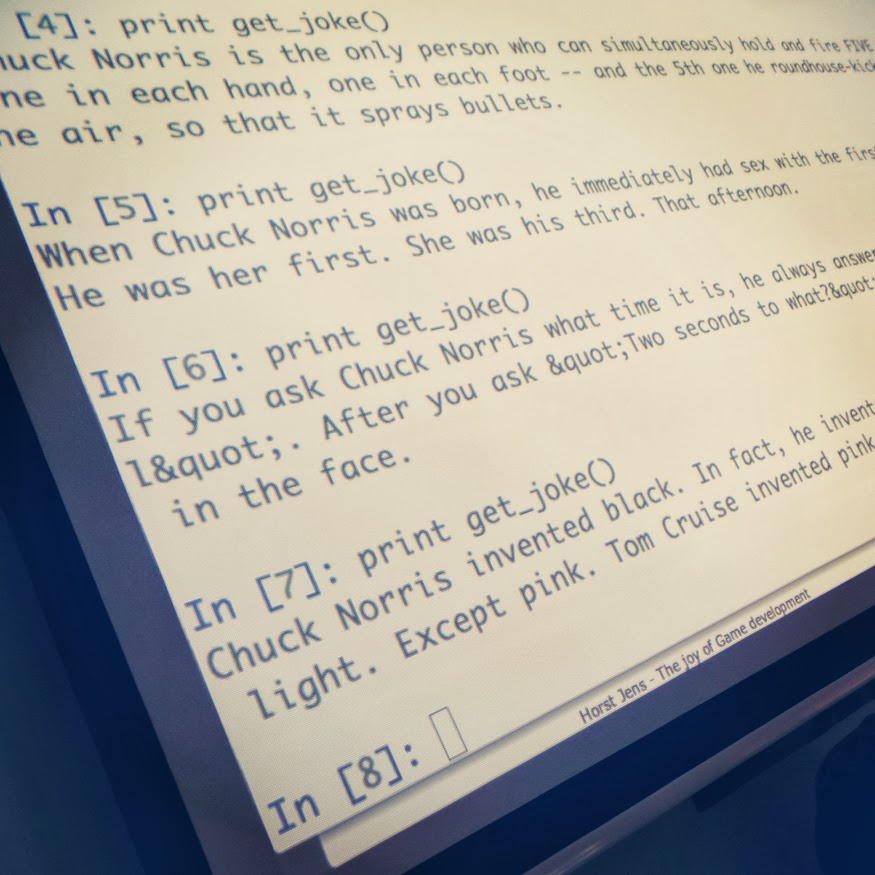
\includegraphics[width=\linewidth]{floor/floor-jokes.jpg} \\
\footnotesize{Output eines Pyladies Treffen. Bildrechte: [1]} 
\end{center}
\subsection*{Fachbegriffe}

~~~\href{https://twitter.com/pyladies_vie}{\textbf{Pyladies Vienna} [1]} steht für Python Ladies, eine Selbstlerngruppe für die Programmiersprache  \textit{Python [3]}, speziell für Frauen. \\

\href{http://python.org}{\textbf{Python} [3]} einfach zu erlernende, Allzweck-Programmiersprache. Wird in den Programmierkursen der Firma \href{http://spielend-programmieren.at}{spielend-programmieren [4]} eingesetzt. \\

\href{http://de.wikipedia.org/wiki/Community_Management}{\textbf{Community Manager}} betreut die Gemeinschaft (Community) im Internet. Kümmert sich z.B. für eine Spielefirma um die Anliegen der im Internet organisierten Fans eines Computerspiels. \\

\textbf{Startup} junges Unternehmen. \\

\textbf{Developer evangelist} versucht Programmierer für eine Firma oder Technologie zu begeistern. \\

\href{https://de.wikipedia.org/wiki/Gamification}{Gamification, gamified learning} versucht die Belohnungsmechanismen und die Motivation von (Computer)spielen auf andere Bereiche zu übertragen, in diesem Fall Lernen. Ein Beispiel dafür sind die Punkte und Badges (Abzeichen) die man bei der Website \href{http://khanacademy.org}{KhanAcademy.org} erwerben kann. \\
 
\textbf{html} steht für Hyper Text Mark Up Language. Seitenauszeichnungssprache. Damit werden Websiten beschrieben, z.B. Überschriften, Tabellen, Hyperlinks etc. \\

\textbf{Css} steht für Cascading Style Sheet. Ermöglicht es, Webseiten (html) optisch zu gestalten (Farben, Layout) \\

\textbf{Bugs fixen}: Programmfehler (so genannte Bugs) reparieren \\


\subsection*{Download, Feedback:}
\footnotesize{
Download: Ordner \texttt{floor} \Mundus\ \href{http://spielend-programmieren.at/risjournal/001}{spielend-programmieren.at/risjournal/001}\\
Startseite:\\
\href{http://spielend-programmieren.at/de:ris:001}{spielend-programmieren.at/de:ris:001}\\ 
\Letter\:  floordrees@gmail.com \\}
\normalsize
 

\subsection*{Lizenz, Quellen}

\begin{wrapfigure}{l}{2.0cm}

\includegraphics[width=2cm]{floor/ccbysa88x31.png}
%
\includegraphics[width=2cm]{horst2011mitdoppeltux.jpg}
%\begin{center}
%\footnotesize{Horst JENS}
%\end{center}
\end{wrapfigure}
Dieses Material steht unter der Creative-Commons-Lizenz Namensnennung - Weitergabe unter gleichen Bedingungen 4.0 International. Um eine Kopie dieser Lizenz zu sehen, besuchen Sie \url{http://creativecommons.org/licenses/by-sa/4.0/deed.de}.

\textbf{Quellen:} \\
{[}1{]} \href{https://twitter.com/FloorDrees}{FloorDrees} \\
bzw.    \href{https://plus.google.com/+FloorDrees/about}{plus.google.com/+FloorDrees} \\
{[}2{]} \href{https://twitter.com/pyladies_vie}{twitter.com/pyladies\_vie} \\
bzw: \href{http://www.meetup.com/pyladies-vienna}{meetup.com/pyladies-vienna} \\
{[}3{]} \href{http://python.org}{python.org} \\
{[}4{]} \href{http://spielend-programmieren.at}{spielend-programmieren.at} \\
{[}5{]} \href{http://www.checkio.org/}{www.CheckiO.org} \\
{[}6{]} \href{http://rubyrogues.com/}{rubyrogues.com} \\
{[}7{]} \href{http://objectsonrails.com/}{objectsonrails.com} \\
{[}8{]} \href{http://www.confidentruby.com/}{confidentruby.com} \\
{[}9{]} \href{http://kytrinyx.com/}{kytrinyx.com} 

\end{multicols}
%\SepRule
%-----------------------------------------------------------
\end{document}
